\chapter{Related Work}

\section{Cityscapes}
\label{ch:cityscapes}
Cityscapes \cite{cordts2016cityscapesdatasetsemanticurban} is a real-world dataset containing over 5000 different semantically labeled images from large German cities. These images are taken out of a car with the goal of adapting the camera angle of self-driving cars. 

The train and validation labels are publicly available, while the test labels are private. Next to semantic segmentation also 2d bounding boxes and depth maps are provided in the "fine" format. Various parts of the dataset were later extended by synthetically generated weather condition scenes, e.g., different strengths of rain and fog. 

Because of the dataset's size, availability, and realism, parts of the dataset have been selected as my test data set for the object detection tasks. \cite{cordts2016cityscapesdatasetsemanticurban} 

\section{Carla}
\label{ch:carla}
The CARLA simulator \cite{dosovitskiy2017carlaopenurbandriving} is an open-source platform for research into autonomous driving and training. It provides realistic environments for testing and developing autonomous vehicle systems and offers features such as the simulation of urban driving scenarios, different weather conditions, and complex traffic situations. CARLA has different maps of urban environments for enough variety, including detailed street plans, traffic signals, buildings, and pedestrians. These environments are designed to accurately simulate real-world driving conditions. Users can create and customize driving scenarios to test specific behaviors of autonomous vehicles. This involves the ability to control weather conditions, lighting, and traffic patterns.
CARLA has many sensors commonly used in autonomous vehicles, such as cameras, LiDAR, GPS, IMU (Inertial Measurement Unit), Depth Maps, Semantic Segmentation, and RADAR \cite{dosovitskiy2017carlaopenurbandriving}. These sensors can be attached to the simulated vehicle to collect data for perception and navigation tasks and be controlled via a Python API. \cite{dosovitskiy2017carlaopenurbandriving}
In this paper, the presented pipeline leverages the CARLA python package to allow importing synthetic data directly from CARLA into the pipeline.

\section{Synthehicle}
\label{ch:synthehicle}
Synthehicle \cite{Herzog_2023_WACV} is a synthetic dataset optimized for "multiple vehicle tracking and segmentation in multiple overlapping and non-overlapping camera views." The cameras capturing the cars are placed at high positions, like on traffic lights or next to streets, to simulate traffic control monitoring. The dataset was exported out of CARLA \autoref{ch:carla} and contains 64 different environments in the four different scenes "day", "rain", "dawn", and "night". For all scenarios, 2d and 3d bounding boxen, as well as semantic segmentation, instance segmentation, and depth maps, are provided, all of them formatted as in the Cityscapes format. \cite{Herzog_2023_WACV}
This dataset is the main used set in this thesis and takes part in the object detection tests as well as the temporal and spatial constancy tests.


\section{Multiple Uncertainties for Autonomous Driving Dataset}
\label{ch:muad}
The Multiple Uncertainties for Autonomous Driving Dataset (MUAD) \cite{Franchi2022MUAD} is a synthetic dataset that provides highly situational events to enhance the current detection network from a car's perspective. Therefore, most of the images have realistic weather simulations, trying to recreate the real-world counterparts.

For this work, especially, the annotations are used as an alternative to the Synthehicle \autoref{ch:synthehicle} ones. The dataset consists of around 4000 images, split into training and validation sets. Each image is annotated with its segmentation, bounding boxes, and depth maps, making it a viable first-person test set for the different modules of the presented diffusion pipeline. \cite{Franchi2022MUAD}



\section{ALDM - Adversarial Supervision Makes \\ Layout-to-Image Diffusion Models Thrive}
\label{ch:aldm}
Adversarial Supervision Makes Layout-to-Image Diffusion Models \cite{li2024aldm} is an alternative architecture to force Latent Diffusion Models (LDM) to solve Layout-to-Image tasks next to ControlNets (it is built on top of the ControlNet code) \autoref{ch:controlnet}. The core idea is instead of freezing the LDM weights to add an "adversarial game between the UNET \cite{ronneberger2015unetconvolutionalnetworksbiomedical} and the segmenter" \cite{li2024aldm} and unroll generated noisy images later.

The training process is split into three parts: a slightly adjusted version of the "Traditional DM Training"\cite{li2024aldm}, described in \autoref{sec:latent_diffusion_models}, the "adversarial supervision via a segmenter-based discriminator"-part \cite{li2024aldm} to align on the ground through semantic segmentation and the "multistep unrolling strategy"\cite{li2024aldm} to guide the model during generation.

The first step is the "Traditional DM Training",\cite{li2024aldm} but instead of just training the UNET \cite{ronneberger2015unetconvolutionalnetworksbiomedical} with the goal of noise reduction on the latent image, the semantic segmentations are also added at this training step. This allows more accurate noise prediction, leading to better output quality and more correctness regarding the semantic segmentation labels \cite{li2024aldm}. 

For the "adversarial supervision via a segmenter-based discriminator"-party a segmenter, in the ALDM case, the UperNet \cite{xiao2018unifiedperceptualparsingscene}, is trained alongside the UNET \cite{ronneberger2015unetconvolutionalnetworksbiomedical} to distinguish "fake" pixels from "real" ones. The idea is that each pixel should be mapped to its ground truth label; if that is not possible, it is added to a "fake" class - this idea is denoted by a Cross-Entropy Loss function, which is used for such multi-class semantic segmentation problems \cite{sushko2021needadversarialsupervisionsemantic}:

\begin{align} \label{eq:discriminator-loss}
\mathcal{L}_{\text{Dis}} &= -\mathbb{E}\left[ \sum_{c=1}^{N}\gamma_c
 \sum_{i,j}^{H \times W} y_{i,j,c} \log \left(\text{Dis}(x_0)_{i,jc}\right)
\right] 
-\mathbb{E}\left[ \sum_{i,j}^{H\times W}  \log \left( \text{Dis}(\hat{x}_0^{(t)})_{i,j,c=N+1} \right)
\right], 
\end{align}
The first term:

\begin{equation}
    -\mathbb{E}\left[ \sum_{c=1}^{N}\gamma_c
 \sum_{i,j}^{H \times W} y_{i,j,c} \log \left(\text{Dis}(x_0)_{i,jc}\right)
\right]
\end{equation}
describes the cross-entropy loss for real images as a weighted sum over all classes for all pixels and the indicator $y_{i,j,c}$ (1 if pixel $i,j$ is of class $c$ else 0) and the second part 
\begin{equation}
  -\mathbb{E}\left[ \sum_{i,j}^{H\times W}  \log \left( \text{Dis}(\hat{x}_0^{(t)})_{i,j,c=N+1} \right)
\right]  
\end{equation}
calculates the loss for fake images ($N + 1$, because $N$ classes and $1$ "fake" class). In summary, for real images, it calculates the weighted cross-entropy loss over all classes and pixels, encouraging the discriminator to correctly classify each pixel's true class, while for fake images, it calculates the cross-entropy loss for the "fake" class, encouraging the discriminator to identify fake images accurately.

Also, the Diffusion Loss is extended by:

\begin{align} \label{eq:seg-loss}
\mathcal{L}_{\text{adv}} = -\mathbb{E}\left[ \sum_{c=1}^{N}\gamma_c \sum_{i,j}^{H \times W} y_{i,j,c} \log \left(\text{Dis}(\hat{x}_0^{(t)})_{i,j,c}\right)
\right].
\end{align}

Instead of the ground truth label map $x_0$, for the generator/DM minimizing the adversarial loss $\mathcal{L}_\text{adv}$ for the generated image $\hat{x}_0^{(t)})$ is the goal, see \autoref{sec:gan}. The final function

\begin{align} \label{eq:overall-loss}
\mathcal{L}_{\text{DM}} = \mathcal{L}_{\text{noise}} + \lambda_{\text{adv}} \mathcal{L}_{\text{adv}},
\end{align}

is used to train the generator in an adversarial framework with $\mathcal{L}_{\text{noise}}$ describing the Loss function for the denoiser and $\lambda_{\text{adv}}$ as a weighting factor.

The third step, "multistep unrolling strategy"\cite{li2024aldm}, is used to not rely on the model's ability to denoise an image in just one step. The image is denoised multiple times - each new image is again fed into the discriminator to guide the generation even further, also at early denoising steps.

This architecture forms the foundation of this paper's presented pipeline and generates the first draft of the image via an input segmentation map. This thrives from the paper's compliance with the layout condition, which is relevant to the discussed subject. \cite{li2024aldm}

\section{Exploring Generative AI for Sim2Real in Driving Data Synthesis}
\label{ch:exploring_generative_ai_for_sim2real_in_driving_data_synthesis}

This recently published paper \cite{zhao2024exploring} explores and compares different AI generation strategies to convert segmentation-based data into real-world-looking datasets. The three selected methods are Pix2PixHD (GAN-based) \cite{wang2018highresolutionimagesynthesissemantic}, OASIS \cite{sushko2021needadversarialsupervisionsemantic} (GAN-based), and ControlNet (diffusion-based, see \autoref{ch:controlnet}). The qualitative results indicate that Pix2PixHD performs the worst among the evaluated methods, producing blurred and distorted images with black artifacts that lack meaningful structure. OASIS produces images closer to real images but with significant distortions, and both GAN-based methods have problems with occlusion relationships. In contrast, ControlNet accurately represents occlusions and produces better textures, colors, and shapes, although it produces less similar images compared to the Cityscapes dataset images.

Quantitatively, ControlNet performs worse on image quality and perceptual tasks with Cityscapes labels, likely due to the superior design of the GAN-based methods, which include a loss in feature matching and content-based regularization. However, ControlNet shows better robustness and generalization. ControlNet's diffusion-based process helps avoid high-frequency distortions and checkerboard patterns, which are common in GAN outputs. Although not all models can replicate the exact color information of CARLA-generated images, ControlNet's results highlight its potential for improved texture and structural accuracy when generating synthetic data.

One of the main differences between this thesis and the one presented is the focus on object detection as well as fine-tuning. Additionally, this paper includes special weather conditions, allowing for a more focused evaluation in challenging settings. Another aspect is the use of ALDM in this thesis and the approach to combine it with other information, particularly depth, to observe the outcomes. The results from the paper "Exploring Generative AI for Sim2Real in Driving Data Synthesis" were one of the reasons for this paper to focus on diffusion-based algorithms \cite{zhao2024exploring}.

\section{Yolo and YoloX}
Yolo \cite{redmon2016lookonceunifiedrealtime} is an object detection neuronal network that performs object detection and object identification via a pre-trained backbone model combined with multiple CNNs and Feed-Forward Neuronal Networks (FNNs/ANNs). The CNN layers are used for detection and authentication, while the FNNs specialize in one of them. Later versions also use anchor bounding boxes next to further progressing backbone technology and a coupled detection head. Anchors are starting points for predicting the bounding boxes of objects, helping the model not to start from the beginning and rather have a form to begin with.


YoloX \cite{yolox2021} is an advanced, anchor-free version of Yolo that uses a multi-head (see \autoref{fig:yolox_multi_head}) instead of a single-head approach to minimize convergence time. YoloX is shipped in 7 different versions, each of them with a different number of parameter sizes, making the smallest one especially attractive for less powerful hardware. It originates from the Yolo v3 because making this version anchor-free is easier than doing it with future releases where the pipeline depends more on them. For the current models, the Yolo v5 backbone models were used. In tests, YoloX outperforms its Yolo counterparts by a small margin \cite{yolox2021}, making it one of the most powerful object detection networks. 

The tests ran for this thesis heavily depend on Yolo and YoloX: for object detection and fine-tuning, YoloX-x was used, while object tracking was done by Yolo v8.

\begin{figure}[H]
  \centering
  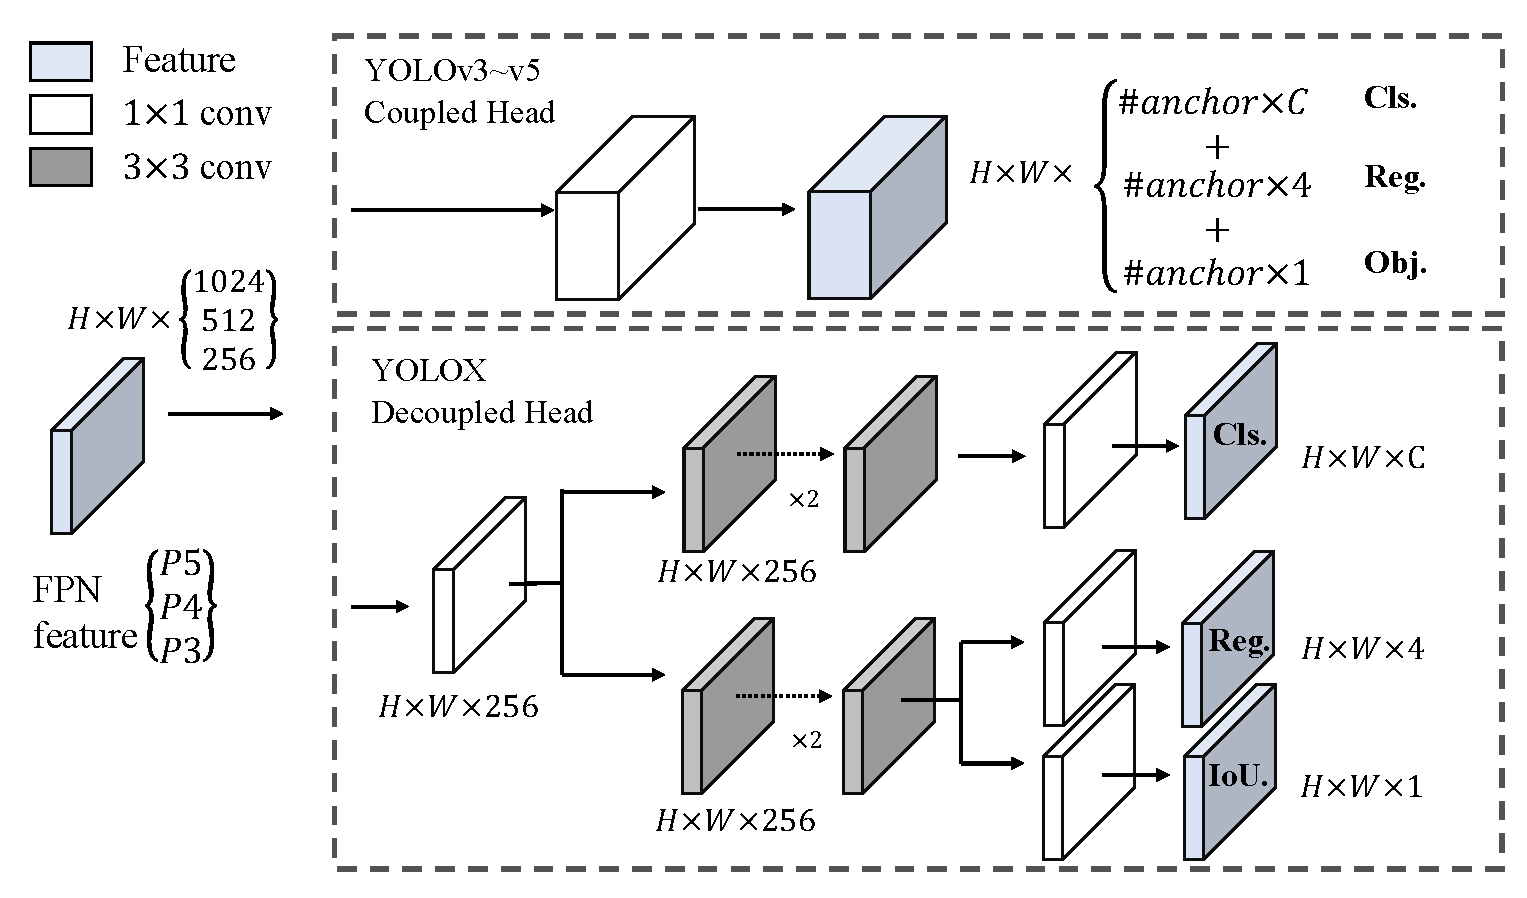
\includegraphics[width=\textwidth]{figures/related_work/yolox-graphic.pdf}
  \caption{Comparison between Yolo and YoloX \cite{yolox2021}. As mentioned, YoloX decouples its heads, allowing more accurate results for classification and bounding box detection.}
  \label{fig:yolox_multi_head}
  \clearpage
\end{figure}